\documentclass[12pt]{extarticle}
\usepackage[english]{babel}
\usepackage{graphicx}
\usepackage{framed}
\usepackage{amsmath}
\usepackage{amssymb}
\usepackage{amsfonts}
\usepackage{enumerate}
\usepackage[utf8]{inputenc}
\usepackage[top=1 in,bottom=1in, left=1 in, right=1 in]{geometry}

\title{Task 2}
\author{s1703913}
\date{April 2019}

\begin{document}

\maketitle
\pagebreak

\section{Task 2.1}
\begin{table}[h!]
\centering
\caption{Analysis of k-NN classification.}
\begin{tabular}{ |p{3cm}|p{3cm}|p{3cm}|p{3cm}|p{3cm}|  }
 \hline
 k&N&Number of errors&Accuracy&Time taken\\
 \hline
 1&3994&145&96.37&6.46 secs\\
 3&3994&141&96.47&6.47 secs\\
 5&3994&145&96.37&6.43 secs\\
 10&3994&147&96.63&6.44 secs\\
 20&3994&166&96.58&6.43 secs\\
 \hline
\end{tabular}
\end{table}

\section{Task 2.2}
\begin{figure}[h!]
\caption{Cross section of decision regions of k-NN with a 2D-PCA plane, where the position of the plane is specified by a point vector. k is the number of nearest neighbours in k-NN.}
\centering
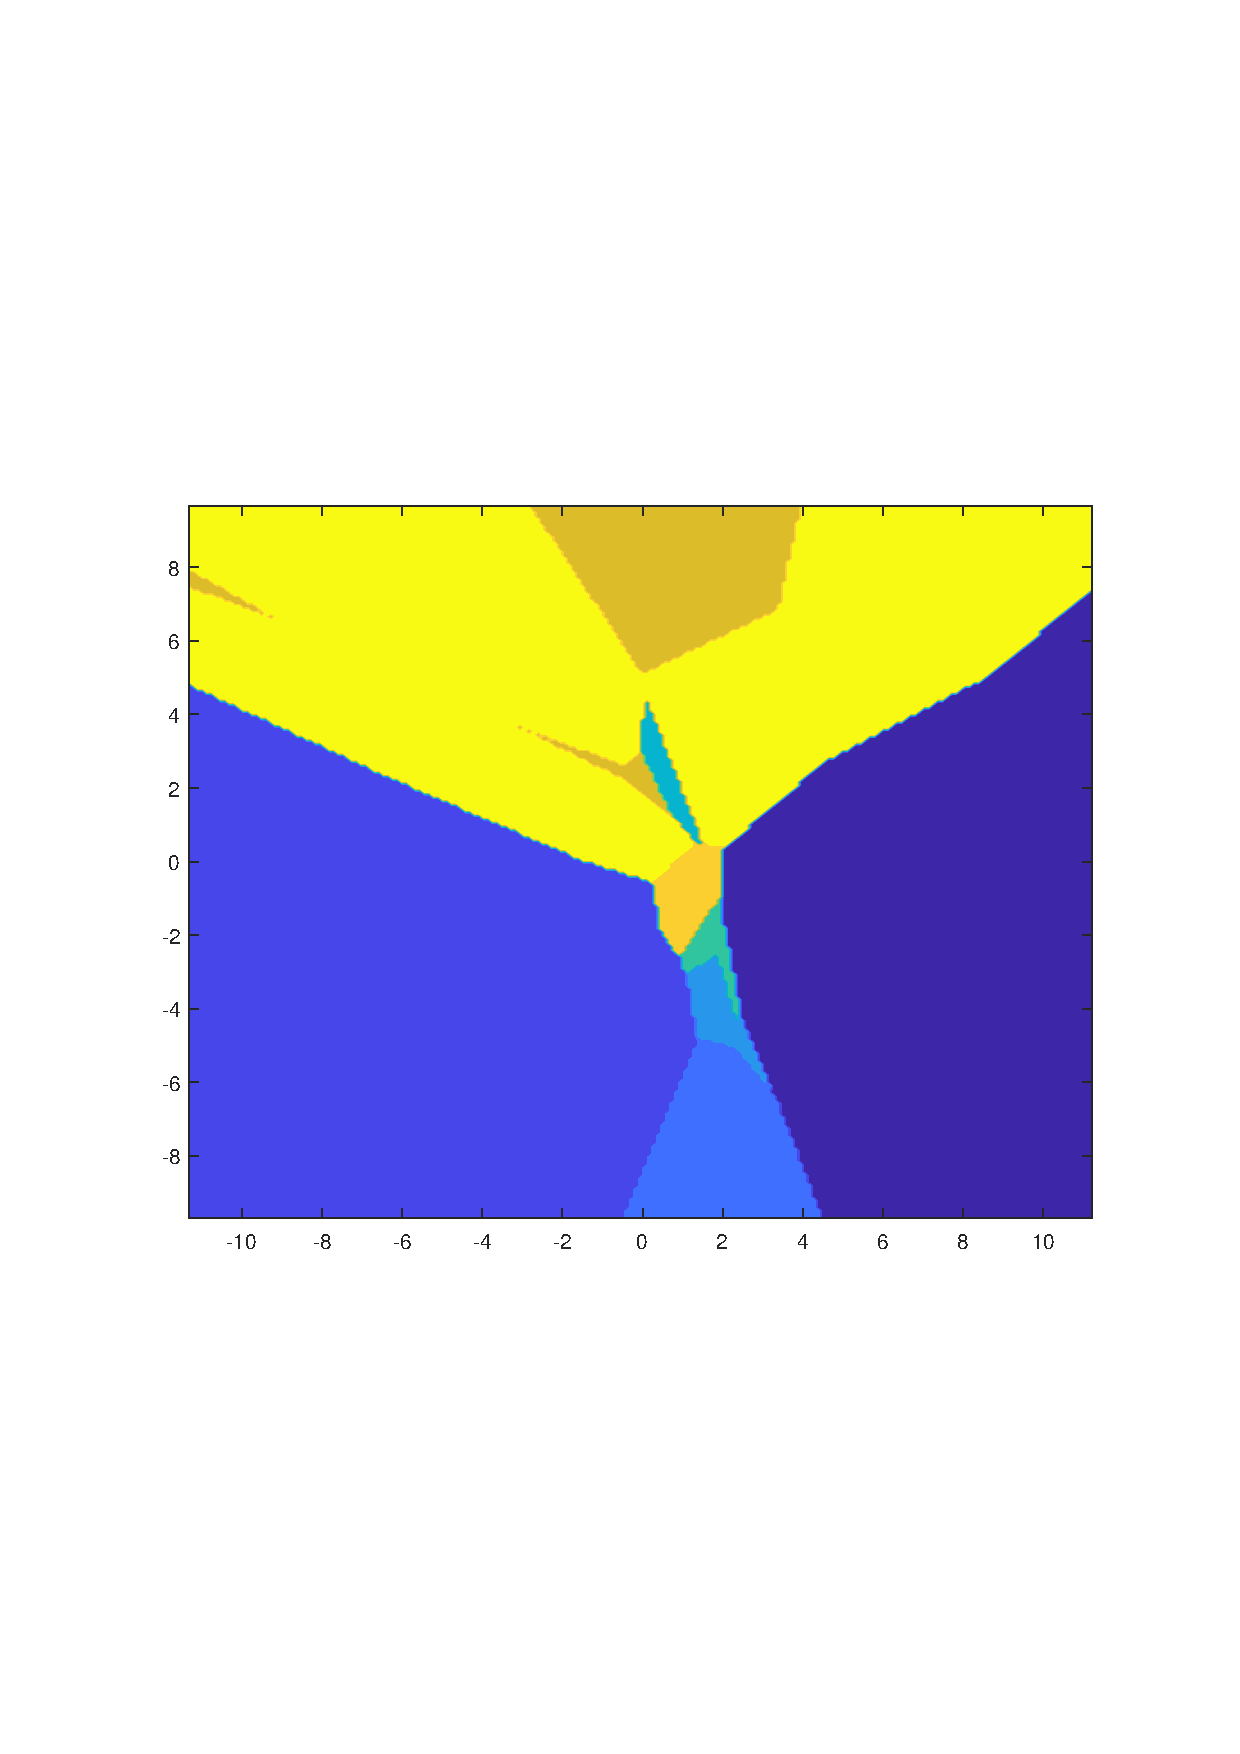
\includegraphics[trim={2cm 7cm 2cm 7cm},height=8cm,width=8cm]{task2_2_imgs_1}
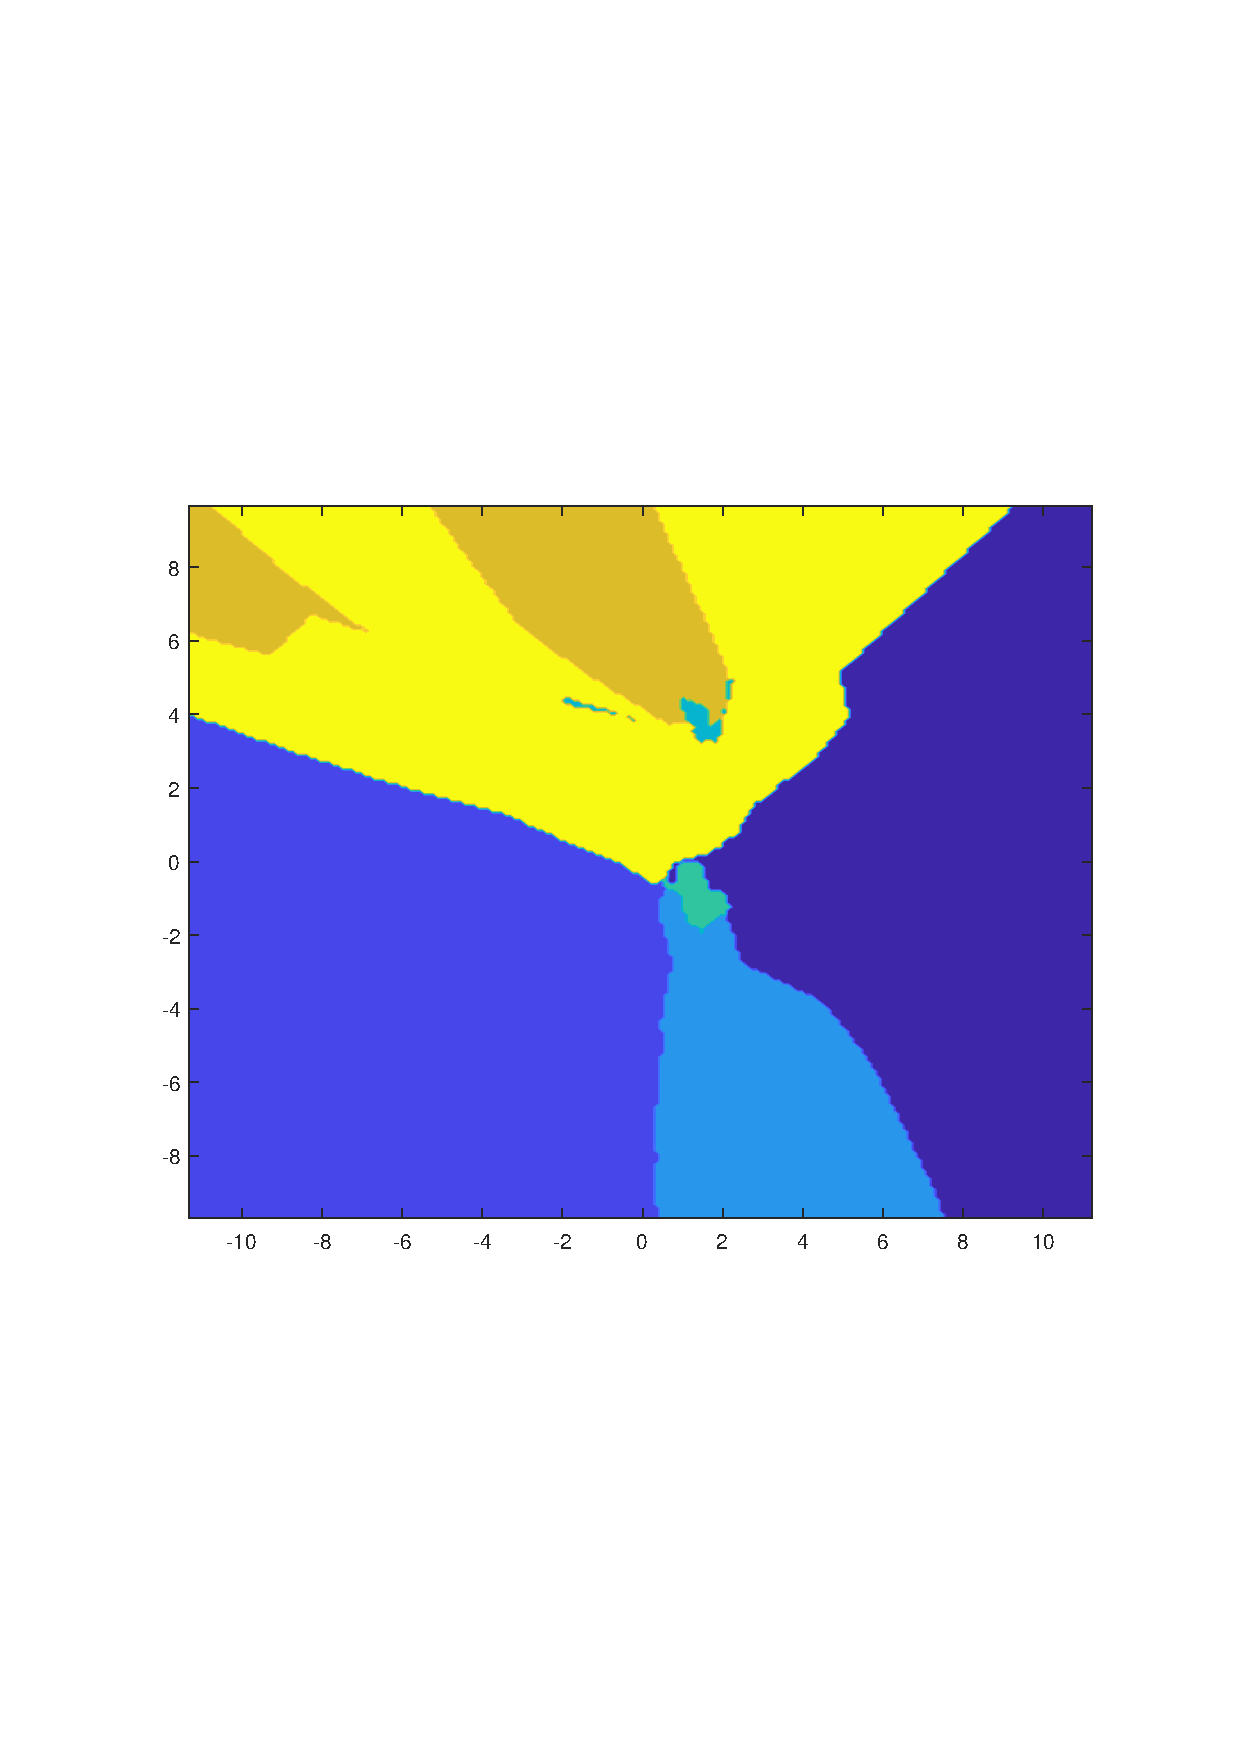
\includegraphics[trim={2cm 7cm 2cm 7cm},height=8cm,width=8cm]{task2_2_imgs_3}
\end{figure}
\begin{center}
 k=1,3
\end{center}
\pagebreak

\section{Task 2.3}
\begin{figure}[h!]
\caption{A contour of Gaussian distribution for each class k = 1,...,10.}
\centering
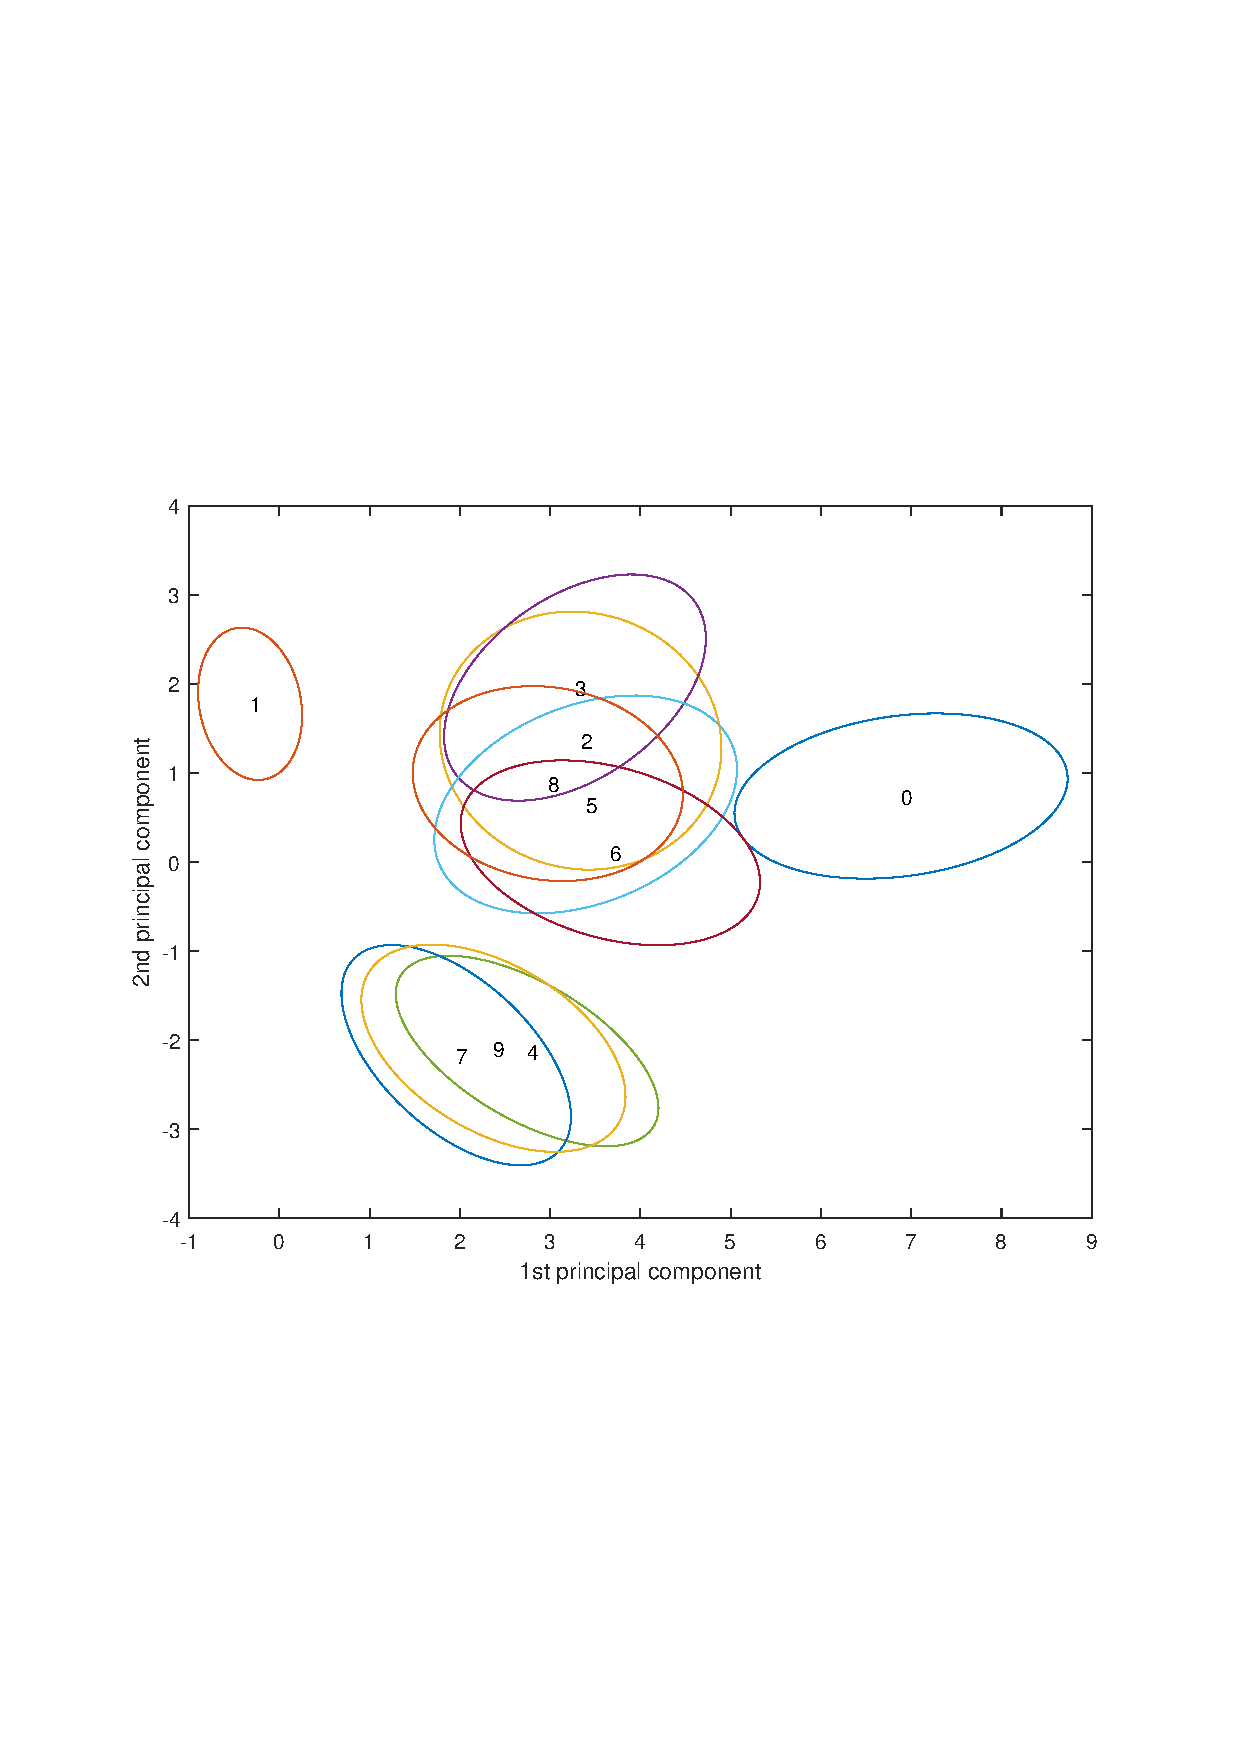
\includegraphics[trim={2cm 7cm 2cm 7cm},height=16cm,width=16cm]{task2_3_img}
\end{figure}
\pagebreak

\section{Task 2.4}
\begin{table}[h!]
\centering
\caption{The correlation on 2D-PCA for each class and for all of the classes (i.e. whole data).}
\begin{tabular}{ |p{3cm}|p{3cm}|  }
 \hline
 Class&Correlation of data points\\
 \hline
 1&-0.2114\\
 2&0.1562\\
 3&0.0593\\
 4&-0.4329\\
 5&0.5979\\
 6&-0.3190\\
 7&0.3186\\
 8&0.5613\\
 9&0.1106\\
 10&0.4654\\
 All data&0.0000\\
 \hline
\end{tabular}
\end{table}

\section{Task 2.5}
\begin{table}[h!]
\centering
\caption{Analysis of Gaussian classification.}
\begin{tabular}{ |p{3cm}|p{3cm}|p{3cm}|p{3cm}|  }
 \hline
 N&Number of errors&Accuracy&Time taken\\
 \hline
 3994&201&94.97&5.25 secs\\
 \hline
\end{tabular}
\end{table}
\pagebreak

\section{Task 2.6}
\begin{figure}[h!]
\caption{Cross section of decision regions of the Gaussian classifiers with a 2D-PCA plane.}
\centering
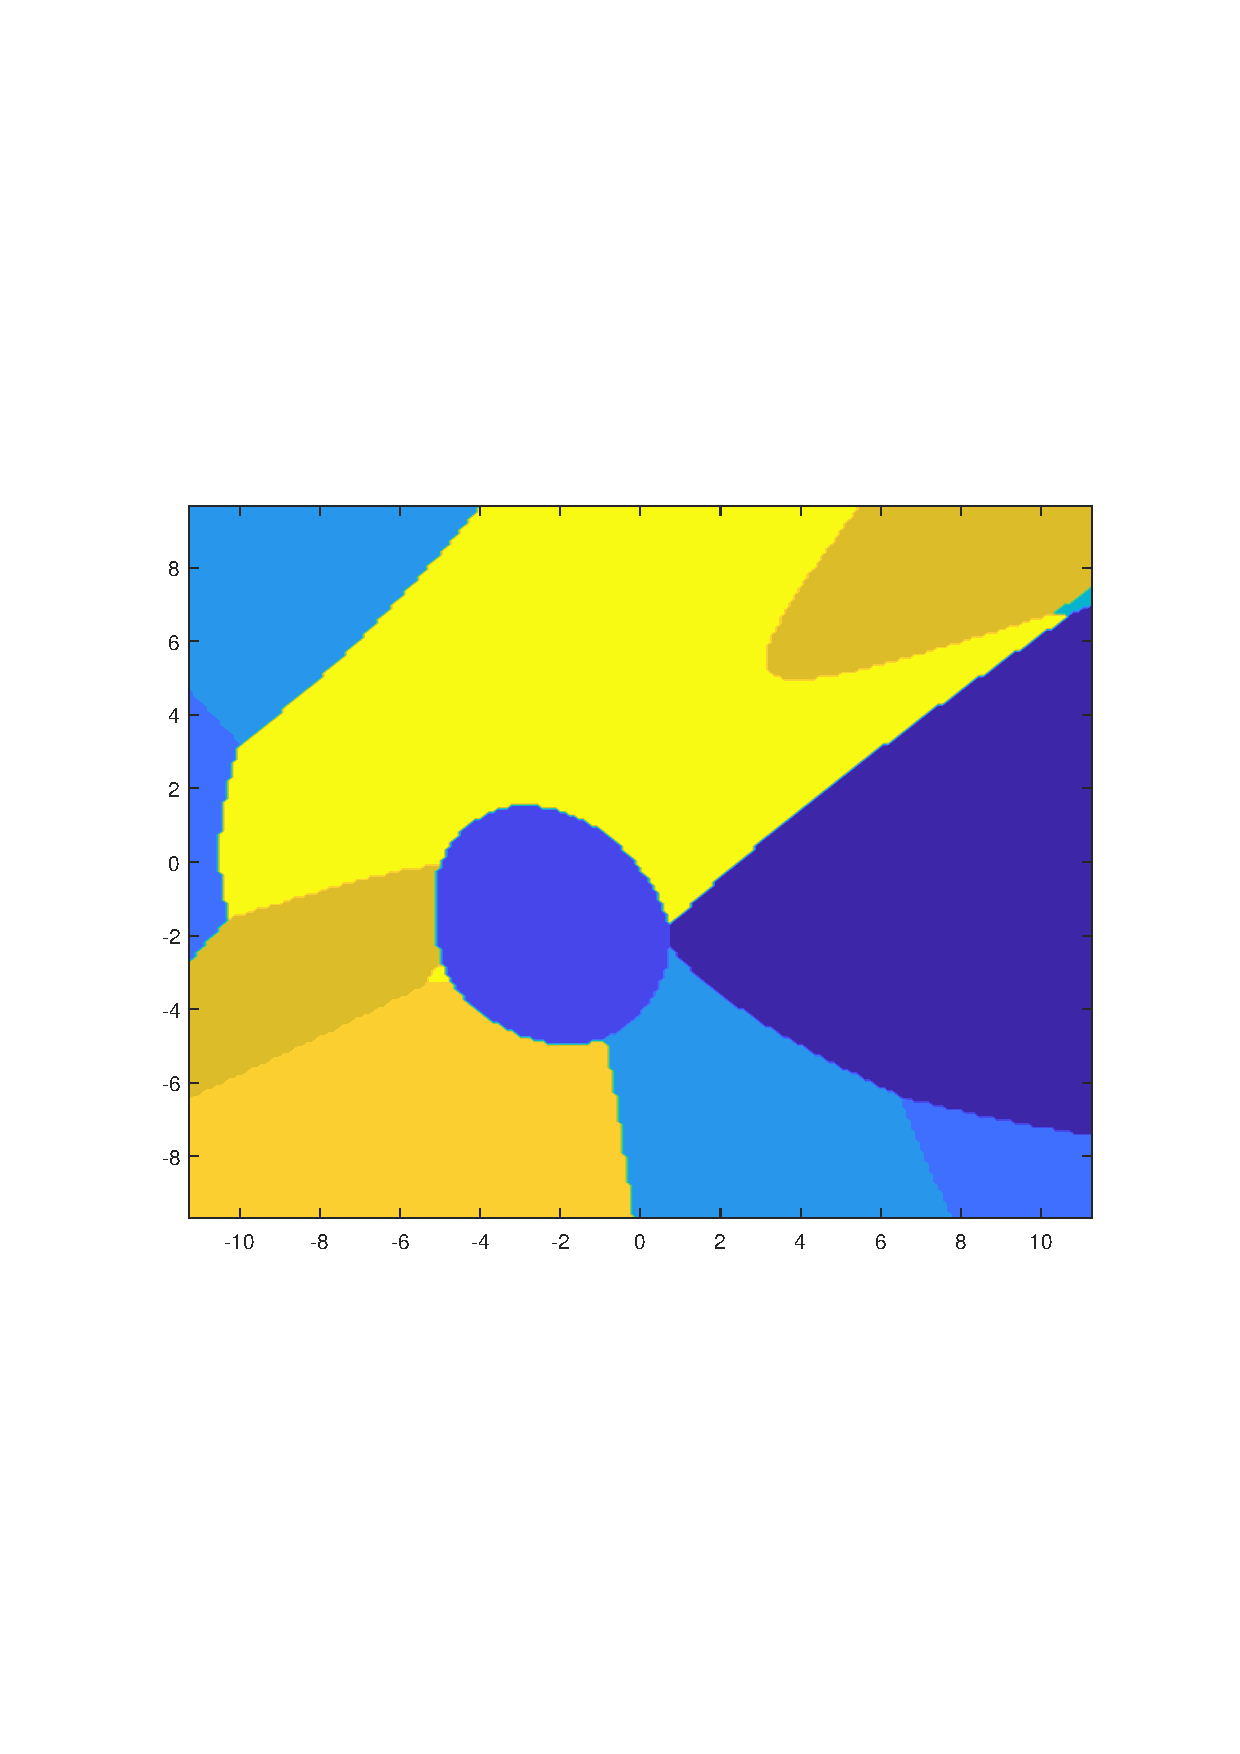
\includegraphics[trim={2cm 7cm 2cm 7cm},height=16cm,width=16cm]{task2_6_img}
\end{figure}
\pagebreak

\section{Task 2.7}
\begin{table}[h!]
\centering
\caption{Accuracy for each percentage of training data respectively used for Gaussian classification. A generally decreasing trend can be observed.}
\begin{tabular}{ |p{3cm}|p{3cm}|  }
 \hline
 Percentage of training data&Accuracy\\
 \hline
 90\%&94.89\\
 80\%&94.92\\
 70\%&94.94\\
 60\%&94.82\\
 50\%&94.87\\
 40\%&94.79\\
 30\%&94.64\\
 \hline
\end{tabular}
\end{table}

\section{Task 2.8}
\begin{table}[h!]
\centering
\caption{Analysis of classification carried out with k-means clustering applied to each class to obtain L Gaussian classifiers per class.}
\begin{tabular}{ |p{3cm}|p{3cm}|p{3cm}|p{3cm}|p{3cm}|  }
 \hline
 L&N&Number of errors&Accuracy&Time taken\\
 \hline
 2&3994&178&95.54&17.03 secs\\
 5&3994&140&96.49&57.82 secs\\
 10&3994&101&97.47&116.83 secs\\
 \hline
\end{tabular}
\end{table}

\end{document}